\section{轴建模过程分析}\label{sec:zhoufengxi}
图\ref{fig:xiaolunzhou}所示的轴零件由一个主视图构成,根据\ref{sec:lijieshitu}节的知识可知一个视图通常是不能够唯一表达物体的。但仔细观察轴零件图的垂直方向的尺寸标注,可以发现垂直方向尺寸标注的一个共同点是均有表示直径的符号$\phi$,由此可知轴零件的各个组成部分都是圆柱体。 基于\ref{sec:taotongjianmo}节套筒零件的三维建模经验,可以采用以下两种方式进行三维建模。

\yaodian{合理清晰的尺寸标注有助于视图表达。}
\subsection{运用叠加方式构建}
从图\ref{fig:xiaolunzhou}中可以直观的看出整个轴零件由三段叠加而成,分别是直径$\phi 6$长3的圆柱体、直径$\phi 8$长35的圆柱体和直径$\phi 16$长2的圆柱体。结果如图\ref{fig:zhoufengxi1}所示。
\begin{figure}[htbp]
\centering
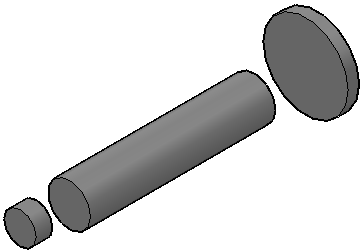
\includegraphics[scale=0.6]{zhoufengxi1.png}
\caption{分段建模}\label{fig:zhoufengxi1}
\end{figure}
\subsection{运用包含关系构建}
轴零件整个都是实体,因此可以将两个轴零件看作这样一种包含关系,即$\phi 16$的圆柱体包含了$\phi 8$和$\phi 6$两个圆柱体的部分实体,$\phi 8$的圆柱体包含了$\phi 6$的部分实体。因此,$\phi 8$圆柱体的长度要加上$\phi 16$圆柱体的长度,故长为37。与此类似,可得$\phi 6$圆柱体的长度则为40。结果如图\ref{fig:zhoufengxi2}所示。
\begin{figure}[htbp]
\centering
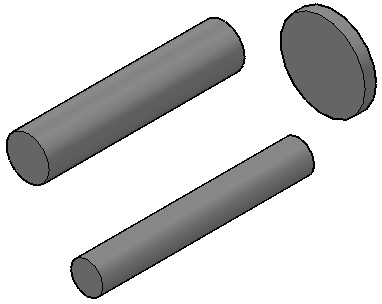
\includegraphics[scale=0.6]{zhoufengxi2.png}
\caption{按包含关系建模}\label{fig:zhoufengxi2}
\end{figure}

对于图\ref{fig:xiaolunzhou}所示的轴零件而言,用分段建模更为直观和直接,但实际中两建模方式并没有优劣之分,应当根据所需建模零件的实际情况灵活地综合运用。
\endinput